\section{Capa Física}

Como mencionamos en la sección anterior, la capa física es la encargada de transmitir la información a través del medio físico mediante lo que se conoce como \textbf{señales}.

\subsection{Bases Teóricas para la Comunicación de Datos}

\begin{definicion}[Señal]
  Definimos una \textbf{señal} como la variación de una magnitud física como un voltaje, corriente, onda electromagnética, etc., en función del tiempo. En este contexto, utilizamos las señales para representar la información que queremos transmitir. Si representamos el valor de la magnitud física como una función del tiempo $f(t)$, podemos modelar el comportamiento de la señal y analizarlo matemáticamente.
\end{definicion}

\begin{definicion}[Componentes de una señal]
  Una señal puede caracterizarse por los siguientes componentes:
  \begin{itemize}
    \item Un \textbf{ciclo} de una señal es la porción de la señal que se repite periódicamente. Es decir, es el conjunto de puntos de la función que se repite a lo largo del tiempo.
    \item El \textbf{periodo} mide el tiempo que tarda una onda en completar un ciclo. Se denota como $T$ y se mide en segundos.
    \item La \textbf{frecuencia} de una señal es la cantidad de veces que se repite un ciclo de la señal en un segundo. Se mide en Hertz (Hz) y es el inverso del periodo de la señal, es decir, $f = \frac{1}{T}$, donde $T$ es el periodo. Es importante destacar que hablar de la frecuencia de una señal solo tiene sentido si la misma es periódica.
    \item La \textbf{amplitud} de una señal es la máxima variación de la magnitud física que representa la señal. Se mide en las mismas unidades que la magnitud física, por ejemplo, voltios para un voltaje o amperios para una corriente.
    \item La \textbf{longitud de onda} es la distancia que recorre la señal en un ciclo completo. Se denota como $\lambda$ y se mide en metros. La longitud de onda está relacionada con la frecuencia y la velocidad de propagación de la señal mediante la ecuación $\lambda = \frac{v}{f}$, donde $v$ es la velocidad de propagación de la señal en el medio.
  \end{itemize}
\end{definicion}

\subsubsection{Análisis de Fourier}

A principios del siglo XIX, el matemático francés Jean-Baptiste Fourier demostró que cualquier función periódica de comportamiento razonable, $g(t)$ con un periodo $T$, se puede construir como la suma de un número (posiblemente infinito) de senos y cosenos:

$$g(t) = \frac{a_0}{2} + \sum_{n=1}^{\infty} a_n \sin\left(2\pi nft\right) + b_n \cos\left(2\pi nft\right)$$

donde $f = \frac{1}{T}$ es la frecuencia fundamental, $a_n$ y $b_n$ son las amplitudes de seno y coseno del $n$-ésimo armónico, y $a_0$ es una constante que representa el valor promedio de la función. Esta representación se conoce como \textbf{serie de Fourier}. Podemos reconstruir la función original $g(t)$ a partir de sus componentes de frecuencia, lo que nos permite analizar y manipular señales de manera más efectiva.

Es posible manejar una señal de datos con una duración finita con sólo imaginar que el patrón completo se repite de manera indefinida. 

Podemos calcular los coeficientes de la serie de Fourier mediante las siguientes ecuaciones:
\begin{align}
  a_n &= \frac{2}{T} \int_{0}^{T} g(t) \sin\left(2\pi nft\right) dt \notag \\
  b_n &= \frac{2}{T} \int_{0}^{T} g(t) \cos\left(2\pi nft\right) dt \notag \\
  a_0 &= \frac{2}{T} \int_{0}^{T} g(t) dt \notag
\end{align}

La relevancia de todo esto para la comunicación de datos es que los canales reales afectan a las señales de manera diferente según las frecuencias que componen la señal. Es más, sabemos con certeza que ningún dispositivo puede transmitir señales a través de un medio físico sin perder cierta potencia en el proceso. 

Si todas las frecuencias de una señal se disminuyen de manera uniforme, la señal se atenúa pero no se distorsiona, lo cual sería ideal. Sin embargo, en la práctica, los canales reales no afectan a todas las frecuencias de manera uniforme, lo que puede llevar a la distorsión de la señal y a la pérdida de información. Por lo tanto, es importante diseñar sistemas de comunicación que puedan compensar estas pérdidas y distorsiones para garantizar una transmisión efectiva de la información.

\subsubsection{Señales de Ancho de Banda Limitado}

\begin{definicion}[Ancho de banda]
  El \textbf{ancho de banda} de un canal de comunicación es la diferencia entre la frecuencia más alta y la frecuencia más baja que puede transmitir el canal sin una atenuación considerable de la señal. Se mide en Hertz (Hz) y es un factor crítico en la determinación de la capacidad de transmisión de datos del canal. Un mayor ancho de banda permite transmitir más información en un período de tiempo determinado (aunque vuelve al sistema susceptible a captar mayor cantidad de ruido e interferencias), mientras que un ancho de banda limitado puede restringir la velocidad de transmisión y afectar la calidad de la señal. En otras palabras, el ancho de banda define el rango de frecuencias que un canal puede manejar de manera efectiva.

  Las señales que van desde cero hasta una frecuencia máxima se llaman señales de \textbf{banda base}. Las que se desplazan para ocupar un rango de frecuencias más altas, como es el caso de todas las transmisiones inalámbricas, se llaman señales de \textbf{pasa-banda}.

  Este concepto también se utiliza para filtrar señales, por ejemplo en las comunicaciones de radio, donde se utilizan filtros de paso de banda para permitir que solo ciertas frecuencias pasen a través del canal, mientras que otras son bloqueadas.

  Es estrictamente necesario diferenciar las dos interpretaciones del término en este contexto: el \textbf{ancho de banda analógico} refiere a la propiedad física del medio descrita anteriormente. En contraste, el \textbf{ancho de banda digital} refiere a la tasa máxima de transferencia de datos de un canal, medida en bits por segundo (bps). Un canal con un mayor ancho de banda analógico permite alcanzar un mayor ancho de banda digital, pero el límite exacto de la tasa de transmisión (bps) estará acotado matemáticamente por el ancho de banda en Hz y el nivel de ruido presente en el medio.
\end{definicion}

\subsubsection{La Tasa de Datos Máxima de un Canal}

La capacidad de transmisión de un canal está restringida matemáticamente por su ancho de banda analógico y por la presencia de interferencias en el medio físico. Existen dos teoremas fundamentales en la teoría de la información que establecen el límite superior de la tasa de datos, diferenciando entre canales ideales y canales con ruido.

\begin{teo}[Teorema de Nyquist]
En un canal ideal (libre de ruido) con un ancho de banda finito $B$, la señal filtrada puede reconstruirse por completo tomando exactamente $2B$ muestras por segundo. Si la señal transmitida consta de $V$ niveles discretos, la tasa de datos máxima está dada por:
$$C = 2B \log_2(V)$$
donde $C$ es la capacidad máxima del canal en bits por segundo (bps), $B$ es el ancho de banda en Hertz (Hz) y $V$ es la cantidad de niveles de señal discretos (cantidad de simbolos distintos que se pueden transmitir).
\end{teo}

El teorema de Nyquist demuestra que, en ausencia de ruido, si se pasa una señal cualquiera a través de un filtro pasa-bajas con un ancho de banda $B$, la señal filtrada se puede reconstruir por completo tomando sólo $2B$ muestras por segundo.

\begin{teo}[Teorema de Shannon]
En un canal real sujeto a ruido aleatorio (ruido térmico), la capacidad máxima de transmisión depende de la relación entre la potencia de la señal y la potencia del ruido. La tasa de datos máxima está dada por:
$$C = B \log_2\left(1 + \frac{S}{N}\right)$$
donde $C$ es la capacidad máxima en bits por segundo (bps), $B$ es el ancho de banda en Hertz (Hz), $S$ es la potencia de la señal y $N$ es la potencia del ruido. La relación $\frac{S}{N}$ se conoce como la relación señal a ruido.
\end{teo}

Debido a la gran variación de la relación señal a ruido, en la práctica se expresa en una escala logarítmica utilizando decibeles (dB), mediante la fórmula:
$$\text{SNR}_{\text{dB}} = 10 \log_{10}\left(\frac{S}{N}\right)$$

El teorema de Shannon establece la cota superior teórica para la transferencia de información en cualquier canal sujeto a ruido aleatorio.

\subsection{Medios de Transmisión Guiados}

El propósito de la capa física es transportar bits de una máquina a otra a través de un medio. Los medios de transmisión guiados confinan la señal dentro de un conducto físico y sólido, como el alambre de cobre o la fibra de vidrio.

\subsubsection{Medios Magnéticos}

Una forma de transferir datos consiste en escribirlos en un soporte de almacenamiento magnético u óptico (como cintas de alta densidad o discos físicos) y transportar dicho soporte físicamente a la máquina de destino. 

Este método posee una \textbf{latencia} extremadamente alta (el tiempo de transporte físico se mide en horas o días), pero su \textbf{ancho de banda efectivo} es destacable, pudiendo alcanzar tasas equivalentes a cientos de Gigabits o Terabits por segundo si se transportan grandes volúmenes de datos físicamente de una sola vez.

\subsubsection{Par Trenzado}

El par trenzado es el medio guiado más antiguo y de uso más extendido. Consiste en dos cables de cobre aislados, típicamente de 1 milímetro de grosor, entrelazados en forma helicoidal, de manera análoga a la estructura de una molécula de ADN. 

Dos cables paralelos actúan como una antena. Al trenzarlos, las ondas electromagnéticas emitidas por los cables se cancelan mutuamente, reduciendo la radiación y mejorando significativamente la inmunidad frente al ruido externo. La señal se transmite típicamente como una diferencia de voltaje entre ambos cables. Se pueden tender varios kilómetros de par trenzado sin necesidad de amplificación, pero en distancias mayores la señal se atenúa demasiado y se requieren repetidores. El ancho de banda depende del grosor del cable y de la distancia que recorre, pero en muchos casos se pueden lograr varios megabits/seg durante pocos kilómetros.

Los enlaces de comunicaciones se clasifican según su direccionalidad en tres modos operativos:
\begin{itemize}
    \item \textbf{Simplex:} La transmisión de datos ocurre en una única dirección fija (el flujo es unidireccional).
    \item \textbf{Half-duplex:} La comunicación puede ocurrir en ambas direcciones, pero de forma alternada, es decir, solamente en una dirección a la vez.
    \item \textbf{Full-duplex:} La comunicación puede ocurrir en ambas direcciones de manera simultánea (requiere mecanismos de cancelación de eco o el uso de múltiples pares).
\end{itemize}

\subsubsection{Cable Coaxial}

El cable coaxial ofrece un mayor ancho de banda y un nivel superior de protección contra interferencias electromagnéticas en comparación con el par trenzado. 

Está compuesto por un alambre central de cobre macizo (núcleo), rodeado por un material aislante. Sobre el material aislante se sitúa un conductor exterior cilíndrico (generalmente una malla de cobre trenzado), el cual a su vez está recubierto por una funda protectora de plástico. El conductor exterior trenzado proporciona un blindaje que bloquea el ruido eléctrico externo y evita la fuga de la señal interna. Esta construcción permite transmitir a velocidades superiores y alcanzar distancias mayores que las soportadas por los pares trenzados convencionales.

\subsubsection{Líneas Eléctricas}

Esta tecnología propone la reutilización de la infraestructura de cableado eléctrico existente dentro de un edificio para el transporte de señales de datos. 

La principal dificultad técnica de las líneas eléctricas radica en la presencia de ruido eléctrico severo, generado por la conmutación y operación de electrodomésticos, y en las variaciones de las propiedades eléctricas de las instalaciones. Para que los datos no interfieran con la distribución de energía, las señales digitales deben modularse y transmitirse en bandas de frecuencia completamente separadas de la corriente eléctrica.

\subsubsection{Fibra Óptica}

La fibra óptica transmite información utilizando la luz como portadora. Un sistema de transmisión óptico consta de tres componentes fundamentales: una fuente de luz (diodo emisor de luz o láser), el medio de transmisión (un núcleo de vidrio o sílice fundido ultradelgado) y un detector (un fotodiodo que convierte los fotones entrantes en pulsos eléctricos).

\begin{itemize}
    \item \textbf{Fundamentos ópticos y propagación:} Este sistema de transmisión tendría fugas de luz y sería inútil en la práctica si no fuera por un principio fundamental de la física. Cuando un rayo de luz pasa de un medio a otro con distinto índice de refracción, el rayo se refracta. Sin embargo, si el rayo incide en el límite entre ambos medios a un ángulo mayor que un cierto valor crítico, la luz no se refracta hacia el exterior, sino que se refleja por completo hacia el interior del primer medio. Este fenómeno se conoce como reflexión interna total. En un cable de fibra óptica, el núcleo de vidrio se recubre con un revestimiento que posee un índice de refracción menor. Esta configuración confina la luz en el interior del núcleo, causando que los rayos reboten en las paredes internas y se propaguen a lo largo del cable sin pérdida de información hacia el exterior.
    
    \item \textbf{Monomodo y Multimodo:}
    \begin{itemize}
        \item \textbf{Multimodo:} Dado que cualquier rayo que incida por encima del ángulo crítico se reflejará internamente, muchos rayos diferentes pueden rebotar en múltiples ángulos (modos) de manera simultánea. Debido a la dispersión modal (los distintos rayos recorren distancias diferentes y llegan al receptor en momentos distintos, ensanchando el pulso original), se restringe su uso a distancias cortas.
        \item \textbf{Monomodo:} Si el diámetro del núcleo se reduce al orden de unas pocas longitudes de onda de la luz, el cable actúa como una guía de ondas. La luz se propaga en línea recta como un rayo único sin rebotar. Emplea láseres de alta precisión, evita por completo la dispersión modal y es el estándar absoluto para enlaces de larga distancia.
    \end{itemize}
    
    \item \textbf{Métodos de empalme:} La conexión entre dos fibras requiere precisión óptica rigurosa. Existen tres métodos:
    \begin{itemize}
        \item \textbf{Conectores:} Se utilizan conectores mecánicos para unir los extremos, facilitando la conexión en paneles, pero introduciendo una pérdida de señal del 10 al 20 por ciento.
        \item \textbf{Empalmes mecánicos:} Alineación rigurosa de los extremos perfectamente cortados de las fibras dentro de un tubo especial. Presentan una pérdida aproximada del 10 por ciento.
        \item \textbf{Fusión:} Consiste en fundir y unir los extremos de las fibras mediante un arco eléctrico. Forma una unión sólida y continua que casi no presenta atenuación en la señal transmitida.
    \end{itemize}
\end{itemize}

\subsection{Transmisión Inalámbrica}

En contraposición a los medios guiados, la transmisión inalámbrica utiliza el espacio libre para la propagación de ondas electromagnéticas.

\subsubsection{El Espectro Electromagnético y Bandas ISM}

Cuando los electrones se mueven, crean ondas electromagnéticas que se pueden propagar por el espacio (incluso en el vacío). La transmisión inalámbrica se basa en la modulación de ondas electromagnéticas. Al conectar una antena del tamaño apropiado a un circuito eléctrico, las ondas electromagnéticas se pueden difundir de manera eficiente y un receptor las puede captar a cierta distancia. Toda la comunicación inalámbrica se basa en este principio. 

En el vacío, todas las ondas electromagnéticas viajan a la misma velocidad sin importar cuál sea su frecuencia. Esta velocidad se conoce como velocidad de la luz, $c \approx 3 \times 10^8$ m/s. La relación entre la velocidad de propagación, la frecuencia y la longitud de onda está dada por la ecuación $c = f \lambda$, donde $f$ es la frecuencia y $\lambda$ es la longitud de onda.

En la siguiente figura se muestra el espectro electromagnético. Las porciones de radio, microondas, infrarrojo y luz visible del espectro se pueden utilizar para transmitir información mediante la modulación de la amplitud, frecuencia o fase de las ondas. La luz ultravioleta, los rayos X y los rayos gamma serían todavía mejores, debido a sus frecuencias más altas, pero son difíciles de producir y de modular, no se propagan bien entre edificios y son peligrosos para los seres vivos. Las bandas que se listan en la parte inferior de la figura son los nombres oficiales de la ITU (Unión Internacional de Telecomunicaciones) y se basan en las longitudes de onda, por lo que la banda LF va de 1 a 10 km (aproximadamente de 30 a 300 kHz). Los términos LF, MF y HF se refieren a las frecuencias baja, media y alta, respectivamente. Está claro que al asignar los nombres nadie esperaba rebasar los 10 MHz, por lo que las bandas más altas se denominaron después como bandas de muy, ultra, súper, extrema y tremendamente alta frecuencia. \textbf{Más allá de eso ya no hay nombres, pero podrían sonar bien las designaciones de increíble, asombrosa y prodigiosamente alta frecuencia (IHF, AHF y PHF).}

\begin{obs}
  Con \textbf{espectro} nos referimos a la representación de la intensidad (amplitud o potencia) de una señal en función de la frecuencia. En otras palabras, el espectro de una señal es una función en el dominio de la frecuencia e indica qué frecuencias están presentes en la señal y con qué fuerza.
\end{obs}

Los rangos de frecuencia más relevantes utilizados en las telecomunicaciones se clasifican de la siguiente manera:

\begin{itemize}
    \item \textbf{Ondas de radio:} Son omnidireccionales (viajan en todas las direcciones) y fáciles de generar. Sus propiedades de propagación son altamente dependientes de la frecuencia. A bajas frecuencias atraviesan obstáculos con facilidad y siguen la curvatura de la Tierra, experimentando una atenuación por pérdida de trayectoria. A frecuencias superiores, viajan en línea recta, rebotan en obstáculos y se refractan en la ionosfera, lo que permite comunicaciones de mayor alcance.
    
    \item \textbf{Microondas:} Operan por encima de los 100 MHz. Viajan en línea recta, lo que permite enfocar la energía en un haz estrecho mediante antenas parabólicas, incrementando significativamente la relación señal a ruido. Sus principales vulnerabilidades son el desvanecimiento por multitrayectorias (causado por refracción atmosférica) y, en frecuencias cercanas o superiores a los 4 GHz, la atenuación severa por absorción de agua (lluvia).
    
    \item \textbf{Infrarrojo:} Ondas no guiadas de corto alcance altamente direccionales. Su característica limitante y definitoria es la incapacidad de atravesar objetos sólidos. Esta restricción física representa una ventaja en el diseño de redes, ya que aísla los sistemas en recintos adyacentes evitando interferencias y elevando la seguridad frente al espionaje.
    
    \item \textbf{Ondas de luz:} Comunicación óptica de espacio libre (típicamente empleando láseres). Ofrece anchos de banda sumamente elevados a bajo costo y sin requerimientos de licenciamiento. Es estrictamente unidireccional y exige una alineación extremadamente precisa. Sus desventajas principales incluyen la dispersión térmica (interferencia por corrientes de convección en el aire) y la atenuación ante condiciones meteorológicas adversas como lluvia o niebla.
\end{itemize}

Dado que el espectro radioeléctrico es un recurso físico finito y susceptible a interferencias cruzadas, su uso se encuentra fuertemente regulado. Sin embargo, existen bandas de frecuencia exentas de licencia, denominadas \textbf{bandas ISM} (Industrial, Científica y Médica), tales como 900 MHz, 2.4 GHz y 5.8 GHz. Cualquier dispositivo puede transmitir en estas bandas, condicionado a restricciones estrictas de potencia máxima y, frecuentemente, a la implementación de técnicas de dispersión de señal para minimizar la interferencia.

\subsubsection{Satélites de Comunicación}

En su forma más simple, podemos considerar un satélite de comunicaciones como un enorme repetidor de microondas en el cielo que contiene varios transpondedores, cada uno de los cuales escucha en cierta porción del espectro, amplifica la señal entrante y después la retransmite en otra
frecuencia para evitar interferencia con la señal entrante. Este modo de operación se llama tubo doblado. Se puede agregar un procesamiento digital para manipular o redirigir por separado los flujos de datos en toda la banda, o el satélite puede recibir información digital y retransmitirla. Esta forma de regeneración de señales mejora el desempeño si se le compara con un tubo doblado, ya que el satélite no amplifica el ruido en la señal que va hacia arriba. Los haces que descienden pueden ser amplios y cubrir una fracción considerable de la superficie de la Tierra, o pueden ser estrechos y cubrir un área de unos cuantos cientos de kilómetros de diámetro.

Nos centraremos en los \textbf{satélites geoestacionarios}, que se encuentran a una altitud de aproximadamente 36.000 km sobre el ecuador. A esta altura, la velocidad angular del satélite coincide con la de rotación de la Tierra, por lo que el satélite parece estar fijo en el cielo desde cualquier punto de la superficie terrestre. Esto permite que las antenas receptoras permanezcan apuntando hacia el mismo lugar sin necesidad de seguimiento. Sin embargo, la distancia considerable introduce un retardo de propagación significativo (aproximadamente 250 ms) y una atenuación notable de la señal. Además, la cobertura de un satélite geoestacionario es limitada a aproximadamente un tercio de la superficie terrestre.

Una propiedad importante de los satélites es que son medios de difusión por naturaleza. Cuesta lo mismo enviar un mensaje a miles de estaciones dentro de la huella de un transpondedor que enviarlo a una sola. Para algunas aplicaciones esta propiedad es muy útil. Por ejemplo, podríamos imaginar un satélite difundiendo páginas web populares a las cachés de una gran cantidad de computadoras dispersas sobre un área amplia. Aun cuando podemos simular la difusión mediante líneas de punto a punto, es probable que la difusión vía satélite sea más económica. Por otro lado, desde el punto de vista de la privacidad, los satélites son un completo desastre: todos pueden escucharlo todo. Es esencial el cifrado cuando se requiere seguridad.

\subsection{Modulación Digital y Multiplexación}

La transmisión de información requiere codificar bits digitales en señales físicas que el medio pueda transportar (modulación) y, frecuentemente, compartir la capacidad total de un mismo canal entre múltiples comunicaciones simultáneas (multiplexación).

\subsubsection{Transmisión en Banda Base}

La transmisión en banda base consiste en la conversión directa de un flujo de datos digitales en variaciones de voltaje o luz que se envían por el medio, ocupando las frecuencias desde cero hasta un límite dado. Para realizar esta conversión se utilizan \textbf{códigos de línea}. Algunos de los códigos de línea más importantes son:

\begin{itemize}
  \item \textbf{NRZ (No Retorno a Cero):} Es la codificación más simple, donde un nivel de voltaje positivo representa un 1 y un voltaje negativo representa un 0. Su principal deficiencia es la falta de recuperación de reloj: una larga secuencia de ceros o unos consecutivos provoca que el receptor a la larga pierda la sincronización y no pueda determinar dónde termina un bit y comienza el siguiente, resultando en errores de interpretación de la señal.
  \item \textbf{NRZI (No Retorno a Cero Invertido):} Es una variante de NRZ que resuelve parcialmente el problema de sincronización. En este esquema, un 1 se representa mediante una transición de voltaje (de alto a bajo o de bajo a alto), mientras que un 0 se representa por la ausencia de transición. Esto garantiza al menos una transición por cada bit 1, pero aún puede haber largas secuencias de ceros consecutivos que provoquen pérdida de sincronización.
  \item \textbf{Codificación Manchester:} Resuelve el problema de sincronización forzando una transición de voltaje en la mitad de cada periodo de bit (de alto a bajo para un 1, y de bajo a alto para un 0). Esta transición funciona como una señal de reloj incorporada. Su desventaja fundamental es que requiere el doble de ancho de banda analógico que NRZ para transmitir la misma tasa de datos.
  \item \textbf{Codificación bipolar:} Utiliza tres niveles de voltaje: positivo, negativo y cero. Un 1 se representa alternando entre los niveles positivo y negativo, mientras que un 0 se representa con el nivel cero. Esto permite la detección de errores mediante la verificación de la alternancia de los niveles de voltaje.
\end{itemize}

A la hora de elegir diseñar la codificación en una transmisión, es fundamental considerar los siguientes aspectos:

\begin{itemize}
  \item \textbf{Eficiencia del ancho de banda:} \\
  Con NRZ, la señal puede alternar entre los niveles positivo y negativo hasta cada 2 bits (en caso de alternar 1s y 0s). Esto significa que necesitamos un ancho de banda de por lo menos $B/2$ Hz cuando la tasa de bits es de $B$ bits/seg. Esta relación proviene de la tasa de Nyquist, por lo tanto no podemos operar el esquema NRZ a una mayor velocidad sin usar más ancho de banda. Por lo general el ancho de banda es un recurso limitado. Entre más altas sean las frecuencias de las señales su atenuación es cada vez mayor, lo que las hace menos útiles, además las señales de frecuencias más altas también requieren componentes electrónicos más rápidos.

  Una estrategia para utilizar el ancho de banda limitado con más eficiencia es usar más de dos niveles de señalización. Por ejemplo, si utilizamos cuatro voltajes podemos enviar 2 bits a la vez como un solo símbolo. Este diseño funcionará siempre y cuando la señal en el receptor sea lo bastante fuerte como para diferenciar los cuatro niveles. La tasa a la que cambia la señal es entonces la mitad de la tasa de bits, por lo que se reduce el ancho de banda necesario. La tasa a la que cambia la señal se denomina \textbf{tasa de símbolo} para diferenciarla de la \textbf{tasa de bits}. La tasa de bits es la tasa de símbolo multiplicada por el número de bits por símbolo.

  \item \textbf{Recuperación de reloj:} \\
  En todos los esquemas que codifican bits en símbolos, el receptor debe saber cuándo termina un símbolo y empieza el siguiente para decodificar los bits de forma correcta. Como ya mencionamos, en la codificación NRZ, largas secuencias de ceros o unos consecutivos pueden provocar que el receptor pierda la sincronización y no pueda determinar dónde termina un bit y comienza el siguiente.

  Los relojes exactos serían útiles para resolver este problema, pero son una solución costosa para un equipo básico. Recordando que vamos a sincronizar bits en enlaces que operan a muchos megabits/seg, por lo que el reloj tendría que variar menos de una fracción de un microsegundo durante la sucesión más larga permitida. Esto podría ser razonable para los enlaces lentos o mensajes cortos, pero no es una solución general.

  Una estrategia es enviar una señal de reloj separada al receptor. Otra línea de reloj no representa mucho para los buses de computadora o los cables cortos en donde hay muchas líneas en paralelo, pero sería un desperdicio para la mayoría de los enlaces de red, ya que si tuviéramos otra línea para enviar una señal, la podríamos usar para enviar datos.

  Para resolver este problema, se utiliza la codificación Manchester, descrita anteriormente. Como ya vimos, esto introduce un nuevo problema: la codificación Manchester requiere el doble de ancho de banda que NRZ para transmitir la misma tasa de bits.
\end{itemize}





\subsubsection{Transmisión Pasa-Banda}

La transmisión pasa-banda regula una onda analógica continua, denominada \textbf{onda portadora}, para transportar la señal digital. Al alterar características de la portadora, la señal se desplaza a un rango de frecuencias superior predeterminado.

\begin{itemize}
    \item \textbf{Técnicas de modulación básicas:} 
    \begin{itemize}
        \item[b)] \textbf{ASK (Modulación por Desplazamiento de Amplitud):} Dos o más niveles de amplitud representan los datos.
        \item[c)] \textbf{FSK (Modulación por Desplazamiento de Frecuencia):} Se utilizan dos o más frecuencias diferentes.
        \item[d)] \textbf{PSK (Modulación por Desplazamiento de Fase):} La fase de la onda portadora se desplaza sistemáticamente en intervalos fijos.
    \end{itemize}
    \begin{figure}[h]
      \centering
      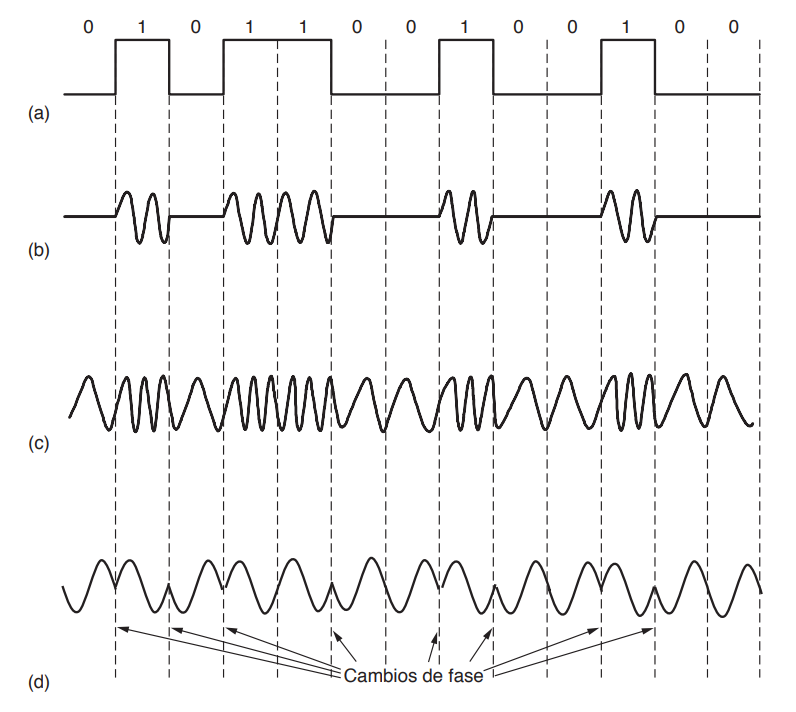
\includegraphics[width=0.7\textwidth]{imgs/2.1.png}
    \end{figure}
\end{itemize}

También tenemos técnicas de modulación más avanzadas, como la \textbf{QAM (Modulación de Amplitud en Cuadratura)} que combina ASK y PSK para transmitir múltiples bits por cada cambio de señal. Los esquemas QAM (como QAM-16 o QAM-64) se representan mediante \textbf{diagramas de constelación}, donde cada punto en el plano representa un estado específico de amplitud y fase, denominado \textbf{símbolo}.

\subsubsection{Multiplexación}

En las comunicaciones resulta muy interesante en terminos de eficiencia utilizar canales de transmisión compartidos por múltiples usuarios. Este estilo de canales, requiere la implementación de técnicas de \textbf{multiplexación}. Para lograr que las señales no se mezclen ni se corrompan entre sí, el canal debe dividirse lógicamente. Las dos dimensiones principales para realizar esta división son la frecuencia y el tiempo.

\begin{itemize}
  \item \textbf{Multiplexación por División de Frecuencia (FDM):}\\
  Aprovecha la transmisión pasa-banda para compartir un canal físico en el dominio de la frecuencia. De manera intuitiva, funciona igual que las emisoras de radio comerciales: todas las estaciones transmiten al mismo tiempo a través del mismo aire, pero cada una sintoniza una frecuencia diferente para que los receptores puedan separarlas.
  \begin{itemize}
    \item \textbf{FDM clásico:} El ancho de banda analógico total del medio se divide en múltiples bandas de frecuencia separadas, asignando cada banda a un usuario o flujo de datos distinto de forma continua. Para evitar que las señales se solapen e interfieran entre canales adyacentes, se introducen pequeños rangos de frecuencia inactivos denominados \textbf{bandas de guarda}.
    \item \textbf{OFDM (FDM Ortogonal):} Una versión más avanzada donde el espectro se divide en un gran número de subportadoras estrechas. A diferencia del FDM tradicional, en OFDM las bandas de las subportadoras se superponen para ahorrar espacio, pero se diseñan matemáticamente ortogonales entre sí para no interferir. Esto elimina la necesidad de bandas de guarda y mejora drásticamente la eficiencia espectral.
  \end{itemize}

  \item \textbf{Multiplexación por División de Tiempo (TDM):}\\
  TDM es una alternativa a FDM. Aquí, los usuarios toman turnos para transmitir. Cada usuario utiliza la totalidad del ancho de banda del canal, pero únicamente durante fracciones de tiempo periódicas denominadas \textbf{ranuras de tiempo}. Se pueden agregar pequeños intervalos de \textbf{tiempo de guarda}, los cuales son análogos a una banda de guarda de frecuencia, para tener en cuenta las pequeñas variaciones de sincronización.
\end{itemize}

